\documentclass{article}
\usepackage{tikz, comment}
\usepackage{pifont}
\usepackage{fontspec}
\usetikzlibrary{arrows, decorations.markings, decorations.pathreplacing}
\begin{comment}
:Title: Not defined yet
:Slug: No name yet

Description Here.........
\end{comment}
\begin{document}\centering 

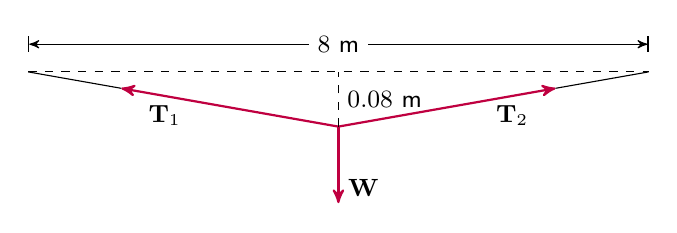
\begin{tikzpicture}[>=latex,xscale=.5*2, yscale=.5*2][font=\sf\small] 

\draw [purple, thick, ->, >=stealth'](0, 0) -- ({2.8*cos(10)}, {2.8*sin(10)})node[black, below, midway, pos=0.8, xshift=0, yshift=0, scale=1]{${\bf T}_2$};

\draw ({2.8*cos(10)}, {2.8*sin(10)}) -- ({4*cos(10)}, {4*sin(10)});

\draw [purple, thick, ->, >=stealth'](0, 0) -- ({2.8*cos(180-10)}, {2.8*sin(180-10)})node[black, below, midway, pos=0.8, xshift=0, yshift=0, scale=1]{${\bf T}_1$};

\draw ({2.8*cos(180-10)}, {2.8*sin(180-10)}) -- ({4*cos(180-10)}, {4*sin(180-10)});

\draw[dashed] ({4*cos(180-10)}, {4*sin(180-10)}) -- ({4*cos(10)}, {4*sin(10)});

\draw[purple, thick, ->, >=stealth'] (0, 0) -- (0, {-(2.8*sin(10)+2.8*sin(180-10))})node[black, right, midway, pos=0.8, xshift=0, yshift=0, scale=1]{${\bf W}$};

\draw[|<->|, >=stealth', yshift=10] ({4*cos(180-10)}, {4*sin(180-10)}) -- ({4*cos(10)}, {4*sin(10)})node[black, fill=white, midway, pos=0.5, xshift=0, yshift=0, scale=1]{$8$ m};

\draw[dashed] (0, 0) -- (0, {4*sin(10)})node[black, right, midway, pos=0.5, xshift=0, yshift=0, scale=1]{$0.08$ m};

%\draw[black, samples=100, smooth, domain=180:190, variable=\t] 
%		plot ({4*cos(10)+1*cos(\t)}, {4*sin(10)+1*sin(\t)}); 

%\draw[black, samples=100, smooth, domain=0:-10, variable=\t] 
%		plot ({4*cos(180-10)+1*cos(\t)}, {4*sin(180-10)+1*sin(\t)}); 

%\node[left, scale=0.6] at ({4*cos(10)+1*cos(185)}, {4*sin(10)+1*sin(185)}) {$\theta$};

%\node[right, scale=0.6] at ({4*cos(180-10)+1*cos(-5)}, {4*sin(180-10)+1*sin(-5)}) {$\theta$};

\end{tikzpicture}
\end{document}